\section{Theorie}

\subsection{Furuata Pendel}
Bei dem Furuta Pendel handelt es sich um ein 1992 von Katsuhisa Furuta entwickeltes nichtlineares Pendel...

Test, ob Umlaute unterstützt werden: ÄÖÜß
Straße (Strasse)
Häuser (Haeuser)

\begin{figure}[htbp]
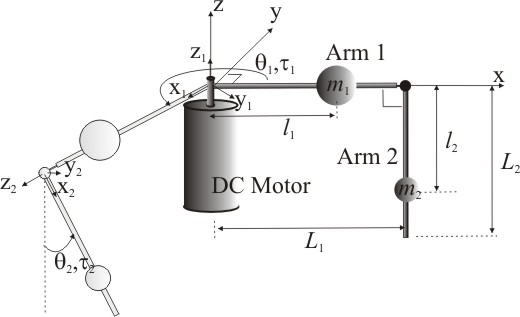
\includegraphics[width=0.8\textwidth]{Grafiken/furuta.jpg}
\caption{Furuta Pendel \colorbox{yellow}{Quelle: Wiki}}
\end{figure}


\begin{equation}
 E_{p1} = 0
\end{equation}

\begin{equation}
E_{k1}=\frac{1}{2}(v^T_{1c}m_1v_{1c}+\omega^T_1J_1\omega_1)=\frac{1}{2}\dot{\theta^2_1}(m_1l_1+J_{1zz})
\end{equation}

\begin{equation}
E_{p2}=gm_2l_2(\cos(\theta_2)-1)
\end{equation}

\begin{eqnarray}
E_{k2}&=&\frac{1}{2}(v^T_{2c}m_2v_{2c}+\omega^T_2J_2\omega_2)\nonumber \\
&=&\frac{1}{2}\dot{\theta^2_1}(m_2L^2_2+(m_2l^2_2+J_{2yy})\sin^2(\theta_2)+J_{2xx}\cos^2(\theta_2))\nonumber \\
&&+\frac{1}{2}\dot{\theta^2_2}(J_{2zz}+m_2l^2_2)+m_2L_1l_2\cos(\theta_2)\dot{\theta_1}\dot{\theta_2}
\end{eqnarray}

\begin{equation}
L=E_k-E_p
\end{equation}

\begin{equation}
\frac{d}{dt}(\frac{\partial L}{\partial\dot{q_i}})+b_i\dot{q_i}-\frac{\partial L}{\partial q_i}=Q_i
\end{equation}

\begin{equation}
\begin{bmatrix}
\tau_1 \\
\tau_2
\end{bmatrix}
=
\begin{bmatrix}
\begin{pmatrix}
\ddot{\theta_1}(J_{1zz}+m_1l^2_1+m_2L^2_1+(J_{2yy}+m_2l^2_2) 						\\
\times \sin^2(\theta_2)+J_{2xx}cos^2(\theta_2))+\ddot{\theta_2}m_2L_1l_2\cos(\theta_2)			\\
-m_2L_1l_2\sin(\theta_2)\dot{\theta^2_2}+\dot{\theta_1}\dot{\theta_2}\sin(2\theta_2)	\\
\times(m_2l^2_2+J_{2yy}-J_{2xx})+b_1\dot{\theta_1}
\end{pmatrix}
\\
\begin{pmatrix}
\ddot{\theta_1}m_2L_1l_2\cos(\theta_2)+\ddot{\theta_2}(m_2l^2_2+J_{2zz})	\\
+\frac{1}{2}\dot{\theta_1}\sin(2\theta_2)(-m_2l^2_2-J_{2yy}+J_{2xx})						\\
+b_2\dot{\theta_2}+gm_2l_2\sin(\theta_2)
\end{pmatrix}
\end{bmatrix}
\end{equation}

\begin{eqnarray}
J_1=
\begin{bmatrix}
J_{1xx} & 0 & 0\\
0 & J_{1yy} & 0\\
0 & 0 & J_{1zz}
\end{bmatrix}
\approx
\begin{bmatrix}
0 & 0 & 0\\
0 & J_{1} & 0\\
0 & 0 & J_{1}
\end{bmatrix}
\nonumber \\
J_2=
\begin{bmatrix}
J_{2xx} & 0 & 0\\
0 & J_{2yy} & 0\\
0 & 0 & J_{2zz}
\end{bmatrix}
\approx
\begin{bmatrix}
0 & 0 & 0\\
0 & J_{2} & 0\\
0 & 0 & J_{2}
\end{bmatrix}
\end{eqnarray}

\begin{eqnarray}
\hat{J_1} &=& J_1 + m_1l^2_1	\nonumber	\\
\hat{J_2} &=& J_2 + m_2l^2_2	\nonumber	\\
\hat{J_0} &=& J_1 + m_1l^2_1 + m_2L^2_1
\end{eqnarray}

\begin{equation}
\begin{bmatrix}
\tau_1 \\
\tau_2
\end{bmatrix}
=
\begin{bmatrix}
\begin{pmatrix}
\ddot{\theta_1}(\hat{J_0}+\hat{J_2}\sin^2(\theta_2))+\ddot{\theta_2}m_2L_1l_2\cos(\theta_2)			\\
-m_2L_1l_2\sin(\theta_2)\dot{\theta^2_2}+\dot{\theta_1}\dot{\theta_2}\hat{J_2}\sin(2\theta_2)+b_1\dot{\theta_1}
\end{pmatrix}
\\
\begin{pmatrix}
\ddot{\theta_1}m_2L_1l_2\cos(\theta_2)+\ddot{\theta_2}\hat{J_2}-\frac{1}{2}\dot{\theta^2_1}\hat{J_2}\sin(2\theta_2)						\\
+b_2\dot{\theta_2}+gm_2l_2\sin(\theta_2)
\end{pmatrix}
\end{bmatrix}
\end{equation}


\colorbox{yellow}{Die folgenden Gleichungen enthalten noch den Fehler, den wir finden sollten.} \\
\colorbox{yellow}{Ich habe die Lösung gerade nicht parat.}
\begin{equation}
\ddot{\theta_1} =
\frac{
\begin{bmatrix}
-\hat{J_2}b_1 \\ 
m_2L_1l_2\cos(\theta_2)b_2 \\ 
-\hat{J^2_2}\sin(2\theta_2) \\ 
-\frac{1}{2}\hat{J_2}m_2L_1l_2\cos(\theta_2)\sin(2\theta_2) \\ 
\hat{J_2}m_2L_1l_2\sin(\theta_2)
\end{bmatrix}^T
\begin{bmatrix}
\dot{\theta_1} \\ 
\dot{\theta_2} \\ 
\dot{\theta_1}\dot{\theta_2} \\ 
\dot{\theta^2_1} \\ 
\dot{\theta^2_2}
\end{bmatrix}
+
\begin{bmatrix}
\hat{J_2} \\ 
-m_2L_1l_2\cos(\theta_2) \\ 
\frac{1}{2}m^2_2l^2_2L_1\sin(2\theta_2)
\end{bmatrix}^T
\begin{bmatrix}
\tau_1 \\ 
\tau_2 \\ 
g
\end{bmatrix} }
{\hat{J_0}\hat{J_2}+\hat{J^2_2}\sin^2(\theta_2)-m^2_2L^2_1l^2_2\cos^2(\theta_2)}
\end{equation}



\begin{equation}
\ddot{\theta_2} =
\frac{
\begin{bmatrix}
m_2L_1l_2\cos(\theta_2)b_1 \\ 
-b_2(\hat{J_0}+\hat{J_2}\sin^2(\theta_2)) \\ 
m_2L_1l_2\hat{J_2}\cos(\theta_2)\sin(2\theta_2) \\ 
-\frac{1}{2}\sin(2\theta_2)(\hat{J_0}\hat{J_2}+\hat{J^2_2}\sin^2(\theta_2)) \\ 
-\frac{1}{2}m^2_2L^2_1l^2_2\sin(2\theta_2)
\end{bmatrix}
\begin{bmatrix}
\dot{\theta_1} \\ 
\dot{\theta_2} \\ 
\dot{\theta_1}\dot{\theta_2} \\ 
\dot{\theta^2_1} \\ 
\dot{\theta^2_2}
\end{bmatrix}
+
\begin{bmatrix}
-m_2l_2\cos(\theta_2) \\ 
\hat{J_0}+\hat{J_2}\sin^2(\theta_2) \\ 
-m_2l_2\sin(\theta_2)(\hat{J_0}+\hat{J_2}\sin^2(\theta_2))
\end{bmatrix}
\begin{bmatrix}
\tau_1 \\ 
\tau_2 \\ 
g
\end{bmatrix} }
{\hat{J_0}\hat{J_2}+\hat{J^2_2}\sin^2(\theta_2)-m^2_2L^2_1l^2_2\cos^2(\theta_2)}
\end{equation}

\begin{eqnarray}
\theta_{1e} &=& 0		\nonumber \\
\theta_{2e} &=& \pi	\nonumber \\
\dot{\theta_{1e}} &=& 0		\nonumber \\
\dot{\theta_{2e}} &=& 0	
\end{eqnarray}

\begin{equation}
\end{equation}

\begin{equation}
\end{equation}

\begin{equation}
\end{equation}

\begin{equation}
\end{equation}

\begin{equation}
\end{equation}

\begin{equation}
\end{equation}

\begin{equation}
\end{equation}

\begin{equation}
\end{equation}

\begin{equation}
\end{equation}
